\documentclass[11pt]{article} % do not change this line
\input{BigDataStyle.txt}      % do not change this line
\usepackage[hidelinks]{hyperref}
\usepackage[export]{adjustbox}
\usepackage{amsmath,amsfonts,amssymb,amsthm,latexsym,graphicx,url,bookmark,enumitem,subcaption}

\emergencystretch=5mm
\tolerance=400
\allowdisplaybreaks[4]

\theoremstyle{plain}
\newtheorem{theorem}{Theorem}[section]
\newtheorem{proposition}[theorem]{Proposition}
\newtheorem{corollary}[theorem]{Corollary}
\newtheorem{lemma}[theorem]{Lemma}
\newtheorem{problem}[theorem]{Problem}

\theoremstyle{definition}
\newtheorem*{remark}{Remark}

\title{Machine Learning for Investor Behaviours on Cryptocurrencies}
\author{Chengkai Lu}

\newcommand{\Programme}{Data Science and Analytics with a Year in Industry}

\newcommand*{\figuretitle}[1]{
  {
    \centering
    \text{#1}
    \par\medskip
  }
}

\begin{document}
\maketitle

\declaration

\begin{abstract}
Cryptocurrencies like Bitcoin and Ripple are becoming popular in these years. They can be obtained through mining or transactions. Every individual cryptocurrency can be transferred directly using a public key in digital wallets. Their price is mostly tied to supply/demand and hard to be interfered by governments. In addition, cryptocurrencies have some dependencies because some of them like Dogecoin can only be bought by some major cryptocurrencies such as Bitcoin and Ethereum in cryptocurrency exchanges.

K-means clustering is a popular unsupervised learning algorithm for grouping unlabelled data. It aims on finding the natural way of separating observations into diffident clusters and is quite popular on the area of marketing for discovering potential customer behaviour. In other words, it might have the ability to discover an implicit pattern on the investors' behaviour.

The concept of deep learning becomes very popular in recent years because of better computation on machines and larger scale of data, and it can predict data more precisely even though the difficulty of explanation. Recurrent Neural Network is a multi-layer neural network with time-series in Deep Learning, and Long Short-Term Memory is one of the most popular one in it because of its capability of eliminating vanishing/exploding gradient problems. It performs well on time-series dataset especially on text and voice recognition. Accordingly, experiment on application of LSTM to the price of different cryptocurrencies may produce some unexpected results.

An implementation of modern algorithms combining nearly pure supply/demand problem is highly possible to capture investors’ investing behaviours. If patterns of investing behaviours are found, the most/least profitable products can be predicted accordingly and be used for investment.
\end{abstract}

\listoffigures
\listoftables

\clearpage

\section*{\hfil Acknowledgement\hfil}



\clearpage

\section{Introduction}
\subsection{Motivation}
\subsection{Aims And Objectives}
\subsection{Project Structure}
\subsubsection{Technologies}
\subsubsection{Programme Structure}
\subsubsection{Report Structure}

\section{Background Research}
\subsection{Correlation Analysis}

In statistics, covariance\eqref{eq:2.1} defines the variability between two individual attributes, which means the level of influence from one feature to another. The numbers correspond to similarity/dissimilarity of the two variables. Positive numbers represent a similar behaviour between them, and vice versa\cite{wiki/cov:2018}.

{
  \begin{equation}
    \label{eq:2.1}
    \tag{2.1}
    {\operatorname {cov} (X,Y)=\operatorname {E} [(X-\mu _{X})(Y-\mu _{Y})]}
  \end{equation}

  \footnotesize
  where:
  \begin{itemize}[label=-, leftmargin=4em, itemsep=0.1em]
    \item ${E}$ is the expectation
    \item ${X, Y}$ are vectors of all the samples
    \item $\operatorname {cov}$ is the covariance
    \item ${\mu}_{X}$ is the mean of X
    \item ${\mu}_{Y}$ is the mean of Y
  \end{itemize}
}

However, if we want to measure the strength of the linear relationship in between, covariance is not enough. We also need to consider the variance in each feature to tell whether the linear relationship is strong. In this case, the correlation was introduced. Correlation is a normalised form of covariance. It restricts the numbers to a certain range which shows how strong the relationship is. The most commonly used correlation coefficient is Pearson correlation coefficient\eqref{eq:2.2}. it is calculated by considering the standard deviation of both groups. This can ensure that dispersion of either attribute does not interfere our identification on the strength of mutual linear relationships\cite{ghall/pcc:2015}.

{
  \begin{equation}
    \label{eq:2.2}
    \tag{2.2}
    \rho _{X,Y}={\frac {\operatorname {cov} (X,Y)}{\sigma _{X}\sigma _{Y}}}
  \end{equation}

  \footnotesize
  where:
  \begin{itemize}[label=-, leftmargin=4em, itemsep=0.1em]
    \item ${\rho}$ is the Pearson correlation coefficient
    \item ${X, Y}$ are vectors of all the samples
    \item $\operatorname {cov}$ is the covariance
    \item ${\sigma}_{X}$ is the standard deviation of ${X}$
    \item ${\sigma}_{Y}$ is the standard deviation of ${Y}$
  \end{itemize}
}

The value of Pearson correlation coefficient is always between -1 and +1. A positive number means a positive linear correlation, and a negative number means a negative linear correlation. The closer the number towards the extremes, the stronger the relationship is. If the number is 0, it means there is no linear correlation among the pair\eqref{eq:2.3}.

\begin{equation}
  \label{eq:2.3}
  \tag{2.3}
  \text{relationship} = 
  \begin{cases} 
    \text{total positive linear correlation} & \text{if } \rho = 1 \\
    \text{positive linear correlation} & \text{if } \rho > 0 \\
    \text{no linear correlation} & \text{if } \rho = 0 \\
    \text{negative linear correlation} & \text{if } \rho < 0 \\
    \text{total negative linear correlation} & \text{if } \rho = -1
  \end{cases}
\end{equation}

\subsubsection{Correlation Matrix}

Given a set of data with multiple attributes, we may want to tell people how these attributes interact with each other. In addition, the result of analysis, especially in a simple regression, may not be reasonable when those features are highly dependent.

To achieve this, we can create a matrix which contains all the correlation coefficient calculated from the expanded equation\eqref{eq:2.4} with a set of given samples.

{
  \begin{equation}
    \label{eq:2.4}
    \tag{2.4}
    {\rho_{xy}={\frac {\sum _{i=1}^{n}(x_{i}-{\bar {x}})(y_{i}-{\bar {y}})}{{\sqrt {\sum _{i=1}^{n}(x_{i}-{\bar {x}})^{2}}}{\sqrt {\sum _{i=1}^{n}(y_{i}-{\bar {y}})^{2}}}}}}
  \end{equation}

  \footnotesize
  where:
  \begin{itemize}[label=-, leftmargin=4em, itemsep=0.1em]
    \item ${\rho}$ is the Pearson correlation coefficient
    \item ${n}$ is the sample size
    \item $x_{i}, y_{i}$ are the single samples indexed with i
    \item ${\bar {x}}={\frac {1}{n}}\sum _{i=1}^{n}x_{i}$ (the sample mean)
    \item ${\bar {y}}={\frac {1}{n}}\sum _{i=1}^{n}y_{i}$ (the sample mean)
  \end{itemize}
}

A correlation matrix is a symmetirc matrix to its main diagonal. The values on the main diagonal always equal to 1 because the attributes are fully dependent on themselves. Table \ref{table:cormat} gives an example of how a correlation matrix looks like.

{
  \begin{table}[ht]
    \centering
    \begin{tabular}{|c|c c c c c|}
      \hline
      Features & f1 & f2 & f3 & f4 & f5 \\ [0.5ex]
      \hline
      f1 & 1 & 0.74 & -0.38 & 0.12 & 0.43 \\ 
      \hline
      f2 & 0.74 & 1 & 0.26 & 0.88 & -0.57 \\
      \hline
      f3 & -0.38 & 0.26 & 1 & 0.61 & 0.59 \\
      \hline
      f4 & 0.12 & 0.88 & 0.61 & 1 & -0.22 \\
      \hline
      f5 & 0.43 & -0.57 & 0.59 & -0.22 & 1 \\ 
      \hline
    \end{tabular}
    \caption{Correlation Matrix}
    \label{table:cormat}
  \end{table}
}

\subsection{Principal Component Analysis}

It is always challenging to analyse a dataset with high-dimensional data points. Due to the curse of dimensionality, which was discovered by Richard Ernest Bellman in 1957, higher-dimensional space increases the difficulties of analysing and organising data exponentially\cite{keogh/cod:2017}. Especially in machine learning, given a certain number of samples, the accuracy of predictions on these samples will increase followed by the rising dimensions to a peak but then gradually drop. This is known as Hughes phenomenon\cite{hughes/itoit:1968}. Figure \ref{fig:hughes} shows how the dimensionality influence the accuracy of predictions.

\begin{figure}[ht]
  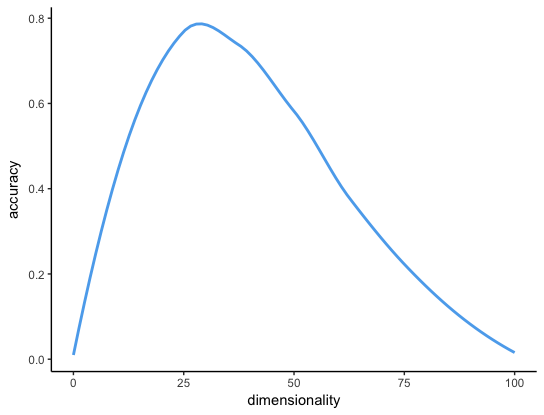
\includegraphics[width=0.8\linewidth, center]{resources/dimensionality.png}
  \caption{Hughes phenomenon}
  \label{fig:hughes}
\end{figure}

In order to reduce the dimensionality, there are two approaches can be implemented:
\begin{itemize}
  \item Feature Selection: To select a subset that is more informative or relevant among all the attributes\cite{hastie/etal:2009}.
  \item Feature Extraction: To generate new features from the initial attributes of existing data\cite{wiki/fs:2018}.
\end{itemize}

The reasons and benefits of executing dimensionality reduction can be summarised as follow:
\begin{enumerate}
  \item Computational efficiency: Fewer features mean less computation on dissimilarity between pairs of data points and lower arithmetic complexity. It also implies less storage usage as the variables in each sample decrease.
  \item Statistical generalisation: By removing noise or irrelevant information from the inputs for building models, the prediction rules can be more general among the datasets.
  \item Better explanation: Visualising a lower-dimensional space is much easier. We can effortlessly illustrate the structure of data when the dimension is lower than 3. Higher-dimensional space will be more challenging to visualise, explain and comprehend.
\end{enumerate}

Principal component analysis(PCA) is a method for feature extraction. It projects features onto a lower-dimensional space. A traditional PCA is a kind of single representation approach as opposed to classification on revealing underlying information in a lower-dimensional space with a linear function. 

In practice, an optimal mapping function is usually non-linear. In order to fit the data in a non-linear way, we can apply a kernel method on top of the traditional PCA, and this is called kernel PCA. It performs a linear PCA mapping in a higher dimensional kernel Hilbert space to provide a better classification. The kernel can be a polynomial function, a radial function or other functions\cite{hessam/kpca:2014}. However, in this project, we will assume that the relationship between the dimensions(cryptocurrencies) are linear and will only use a standard linear PCA to perform the dimensionality reduction.

\subsubsection{Principal Components}

The new features derived are called principal components(PCs). They represent new orthogonal axes in an order based on the amount of information it contains. 

% TODO equations, pseudocode, explanation chart

% \cite{bishop/praml:2006}

\subsection{Clustering}

Clustering, cluster analysis or data segmentation is a non-parametric algorithm in the subtree of unsupervised learning. It is used to separate data into different groups using their dissimilarities(similarities) or possible distributions. Unlike supervised learning, this type of learning algorithms does not have any indicator for assessing the quality of results, and this means that it does not have any meaning or objective itself. Instead, it discovers the distribution of data and uses the definition given by people who have the specific domain knowledge. By giving the rules for partitioning data self-defined meanings, useful information can be obtained and utilised in different domains\cite{hastie/etal:2009}.

In general, clustering can be defined into two types, parametric and non-parametric. A parametric clustering groups the clusters with a a assumed density function which is usually a Gaussian, while a non-parametric one does not have any assumed distribution, it only aims on finding natural groupings within the givien dataset. In this project, we will only focus on the K-means algorithm in non-parametric methods.

K-means clustering and hierarchical clustering are two of the most popular methods in the non-parametric cluster analysis. In K-means clustering, we specify the number of groups we want to classify into. In contrast, hierarchical clustering does not have an initial number of clusters that we want for the result. It instead shows all the possible clusters into a tree structure and allows us to choose the number of clusters we want at the end.

\subsubsection{K-means Clustering}

K-means clustering is a intuitive approach which allows us to separate data points into distinct groups. To implement this, we first need to specify an initial number of clusters - K, and then randomly assign a number(cluster) from 1 to K to each object(data point). In this case, the clusters will have two features\cite{james/itsl:2009}:
{
  \begin{enumerate}
    \item ${C_1}\cup{C_2}\cup...\cup{C_K} = \{{O_1}, {O_2},..., {O_n}\}$
    \item ${C_k}\cap{C_{k^\prime}} = \emptyset \text{,}\quad \text{for} \wedge k \neq k^\prime$
  \end{enumerate}

  \footnotesize
  where:
    \begin{itemize}[label=-, leftmargin=4em, itemsep=0.1em]
      \item ${C_k}$ is the kth cluster
      \item ${O_n}$ is the nth object
    \end{itemize}
}

These properties mean that each single object will be in exactly one cluster and the clusters does not overlap. After this initial setting, we want to optimise\eqref{eq:2.5} the grouping because the previous assignment is just a random initialisation. We want to make sure that the objects are concentrated which means the data point fit the best in the assigned cluster. 

{
  \begin{equation}
    \label{eq:2.5}
    \tag{2.5}
    {{\underset {\mathbf {C_1,...,C_K} }{\operatorname {minimize} }}\left\{\sum _{k=1}^{K}\,{\frac {1}{|C_{k}|}}\,\sum _{ {i} , {i^\prime} \in C_{k}}\sum_{j=1}^{p}(x_{ij}-x_{{i^\prime}j})\right\}}
  \end{equation}

  \footnotesize
  where:
  \begin{itemize}[label=-, leftmargin=4em, itemsep=0.1em]
    \item ${C_k}$ is the kth cluster
    \item ${x_{ij}}$ is the jth attribute of the ith object
  \end{itemize}
}

To fulfil the condition above which is \eqref{eq:2.5}, we can simplify the apporach as below to classify our data points into the multiple clusters\cite{james/itsl:2009}:
{
  \begin{enumerate}
    \item Randomly assign an initial number from 1 to K to each observation.
    \item Iterate over the following steps until the assigned cluster of each observation stops changing:
    \begin{enumerate}
      \item for i in range(1, K): \\
      Compute the centroid of each cluster which is the mean of vectors with the same k(cluster) assigned.
      \item Calculate the distance(Euclidean distance) between each object and each of the clusters.
      \item  Assign the nearest k(cluster) to each observation.
    \end{enumerate}
  \end{enumerate}
}
Figure \ref{fig:kmeans} shows the difference after an optimisation of the cluster assignment. The colors indicate different clusters, and the groups are separated after the implementation of K-means clustering.

\begin{figure}[ht]
  \centering
  \figuretitle{K = 4}
  \begin{subfigure}[b]{0.48\textwidth}
    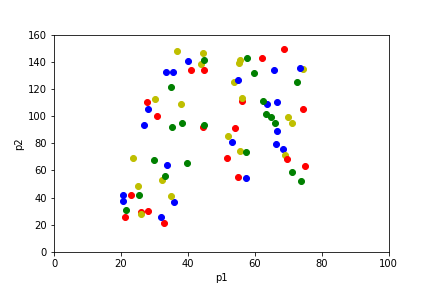
\includegraphics[width=\linewidth, center]{resources/kmeans_before.png}
    \caption{Before Iteration}
    \label{fig:before_iter}
  \end{subfigure}
  \begin{subfigure}[b]{0.48\textwidth}
    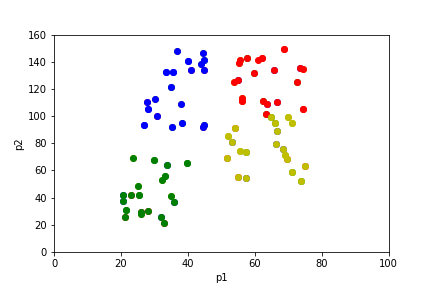
\includegraphics[width=\linewidth, center]{resources/kmeans_after.png}
    \caption{After Iteration}
    \label{fig:after_iter}
  \end{subfigure}
  \caption{K-means Clustering}
  \label{fig:kmeans}
\end{figure}

\subsection{Recurrent Neural Network}
\subsubsection{Long Short-Term Memory}

\section{K-means Clustering on Price Fluctuations}
\subsection{Data Prepocessing}
\subsubsection{Data Formats}
\subsubsection{Normalisation}
\subsubsection{Feature Extraction}
\subsection{Data Analysis}
\subsubsection{Correlation Overview}
\subsubsection{Model Training}
\subsubsection{Shifting Along Timeline}
\subsection{Result}

\clearpage

\section{LSTM on Highest/Lowest Nextday Growth Prediction}
\subsection{Data Prepocessing}
\subsubsection{Data Formats}
\subsubsection{Normalisation}
\subsubsection{Training Set and Validation Set}
\subsection{Data Analysis}
\subsubsection{Activation Functions}
\subsubsection{Parameters}
\subsubsection{Regularisation}
\subsubsection{Loss Function}
\subsubsection{Model Training}
\subsection{Result}
\subsubsection{Back Test}

\section{Conclusion and Evaluation}
\subsection{Performance}
\subsection{Visualisation}
\subsection{Further Work}

\section{Appendix}
\subsection{Programme Usage}

\bibliographystyle{plain}
\bibliography{bibliography}
\end{document}
